\chapter{Component Testing}
\vspace{-12mm}
The components chosen where all Surface-Mount Devices (SMD) in order to minimise the size of the designed PCB. In order to test these components, they were soldered onto pieces of Vero board with male headers so the the component can be connected to a bread board for testing. Any code that was used has been included in the testing procedure and schematics are available in the GitHub repository.

\vspace{-4mm}
\section{Microcontroller} 
\vspace{-4mm}
To test the basic functioning of the micro controller, a schematic was designed with the minimum components required to run the microcontroller and allow for a simple test. The microcontroller will simply turn an LED on and off every 100 mili seconds. This was then implemented on a bread board.

The designed schematic included the necessary components required to run the micro controller. This included an 8MHz external clock, a reset push button, GPIO and debugger pins as well as an LED indicator. As well as the USB debugger setup.

\subsection*{Implemented code:}
\vspace{4mm}
\begin{table}[H]    
    \Centering
    \begin{tabular}{|l|l|}
    \hline
    \textbf{Initialisations:}&\textbf{Main:}\newline\\
    \vspace{-2mm}
    1. GPIO pins for LED's & 1. LED on\\
                           & 2. 100ms delay\\
                           & 3. LED off\\
                           & 4. Item 100ms delay\\
                           \hline
    \end{tabular}
    \caption{Microcontroller code implementation}
\end{table}
    


 



\newpage
\section{Temperature Sensor}
In order to test the temperature sensor. A test would need to be created where the sensors output voltage can be measured and related to the temperature. This test requires that the temperature sensor used for the reference has been calibrated. The reference sensor and the sensor being tested would then be exposed to various temperatures and the results will be tabulated and the sensed temperature can then be calculated using the fact that the sensor output 500mV at 0\degree C, found in the datas heet .Thus at 25\degree C, the Temperature$\mathbf{ = \frac{Vout - 500mV}{gain}}$.

An alcohol thermometer was used as the reference temperature sensor. The thermometer was calibrated by submerging it in an ice bath and reading the temperature after five minutes. The thermometer read 0\degree C, the temperature of ice melting, which meant it was calibrated.

The device was connected following the schematic, but no other components are necessary to run the device. It is suggested in the data sheet to connected a 0.1uF capacitor between $V_D $ and Ground and the gain was set to 10 by using RS = 10\ohm. The chip was then exposed to multiple temperatures while recording Vout using an oscilloscope. Vout was then measured and the actual and sensed temperatures were tabulated below in Table 4.2.
\vspace{5mm}
\begin{table}[H]
\centering
    \begin{tabular}{|c| c| c|}
    \hline
     \textbf{\underline{Actual Temperature (\degree C)}}  & \textbf{\underline{Vout (V})} & \textbf{\underline{Sensed Temperature(\degree C)}}\\
     25 & 0.738 & 23.8 \\
     28 & 0.775 & 27.5 \\
     50 & 0.984 & 48.4 \\
     62 & 1.098 & 59.8 \\
     68 & 1.11  & 61.0 \\
     87 & 1.25  & 75.0 \\
     \hline
    \end{tabular}
    \caption{Temperature sensor results}
\end{table}
The temperature sensor worked with expected accuracy. The MCP1700 data sheet specifies a 2\degree C error for temperatures less than 55\degree C. This accuracy can be seen between 25\degree C-50\degree C. For the results above 55\degree C it can be seen that as the variance increases as the temperature increases.


\newpage
\section{Current Sensor}  
\vspace{-7mm}
In order to create a stable current source for the current sensor, A resitor bank is used for the load. This will allow for the resistance to be changed incrementally by connecting at different points along the resistor bank. Along with a known resistance, applying a constant 10V across the output load will allow for the current through Rs to be known and easily controllable. The INA169 was in its standard configuration. RL was chosen to be 10k\ohm for a gain of 10. For testing purpose a current range of 1mA - 30mA would be tested for and an Rs of 10\ohm. This will allow for sensing at this current range. A lower current range was chosen for testing as low currents are safer and is cheaper to work with. When creating the resistive load bank, it had to be taken note of that the max differential voltage that can be experienced between Vin+ and Vin- is 500mV which outputs an Iout of 500uA. This required that the load needed to have a resistance greater than at least 10 times more than that of the sensing resistor RS.

\vspace{-3mm}
The actual drawn current was simply calculated using $V=IR$. The current measured by the sensor was calculated using $Is =  \frac{Vout*1k\ohm }{10*10k\ohm}$. The output current, voltage and sensed current equations were found in the data sheet.
\vspace{-5mm}
\begin{itemize}
    \item[] $\mathbf{Iout = gm(Vin+ - Vin-)}$, \hspace{10mm} $\mathbf{gm = 1000\frac{uA}{V}}$
    \item[] $ \mathbf{Vout = \frac{Is*Rs*Rl}{1k\ohm}}$  \hspace{33mm} $ \mathbf{Is = \frac{Vout*1k\ohm}{Rs*Rl}}$
\end{itemize}

\vspace{-5mm}
Table 4.3 shows the input and output, as well as the actual and calculated current values that were recorded during the testing. The load resistance in the table refers to the output load being used to create a specific current, not to be confused with RL the load resistor that determines the gain for Vout.

\begin{table}[H]
\centering
    \begin{tabular}{|c| c| c| c|}
    \hline
     \textbf{\underline{Load resistance (\ohm)}}  & \textbf{\underline{Iactual (mA)}} & \textbf{\underline{Vout (V)}} & \textbf{\underline{Is (mA)}}\\
     900 & 10 & 0.98 & 9.8  \\
     800 & 12 & 1.12 & 11.2 \\
     700 & 14 & 1.28 & 12.8 \\
     600 & 16 & 1.47 & 14.7 \\
     500 & 18 & 1.74 & 17.4 \\
     400 & 24 & 2.2  & 22   \\
     300 & 30 & 2.8  & 28   \\
     \hline
    \end{tabular}
     \caption{Current sensor results}
\end{table}
\vspace{-9mm}
The current sensor was able to sense and calculate the output current with an error of about $+- 2mA$. It was found that at resistances of less than 400\ohm  the fraction of the voltage drop across Rs relative to the voltage drop across the load becomes big enough for it to effect the sensed current Is, resulting in a less accurate Vout voltage.

\newpage
\section{MAX485}
\vspace{-8mm}
Termination resistors of RT = 120\ohm for RS485 communication when impedance matching and a 1uF capacitor between $V_{cc}$ and ground for to stabilising the voltage ripple. The MAX485 chip can be tested in its two states, transmitting and receiving. 

\begin{table}[H]
\centering
    \begin{tabular}{|l|l|}
    \hline
            \textbf{\underline{Transmitting:}}&\textbf{\underline{Receiving:}}\\
            1. Connect chip to ground and power          & 1. Connect power and ground\\
            2. Connect \underline{RE} to ground          & 2. Write data to USART TDR\\
            3. Connect DE to 5V                          & 3. Connect \underline{RE} to 5V\\
            4. Supply DI with a PWM signal               & 4. Supply DI with a PWM signal\\
            5. Use oscilloscope to probe pins A and B    & 5. Differential signal is applied to pins A and B\\
                                                         & 6. Use oscilloscope to probe pins RO \\
                                  \hline
    \end{tabular}\
    \vspace{-3mm}
    \caption{Transmission and reception tests}
    \vspace{-13mm}
\end{table}

\subsection{Implementation}
\vspace{-7mm}
When testing the MAX485 the transmission and reception test were both successful indicating a correct setup of the transceiver. The oscilloscope readings of both the transmission and reception tests can be seen below in Figures 4.1-4.4.

\vspace{-1mm}
\begin{table}[H]
    \centering
    \begin{tabular}{|c|c|}
    \hline
    \textbf{\underline{Transmission test}}&\\
    \vspace{-5mm}
      \begin{minipage}[b]{0.45\textwidth}
        \begin{figure}[H]
            \centering
            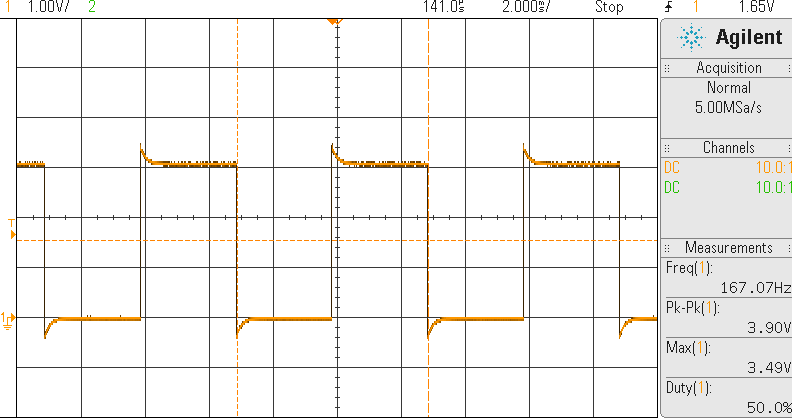
\includegraphics[width=1\textwidth]{max_trans_signal.png}
            \vspace{-8mm}
            \caption{\small{Signal to be transmitted}}
        \end{figure}
      \end{minipage}
       &   
      \begin{minipage}[b]{0.45\textwidth}
        \begin{figure}[H]
            \centering
            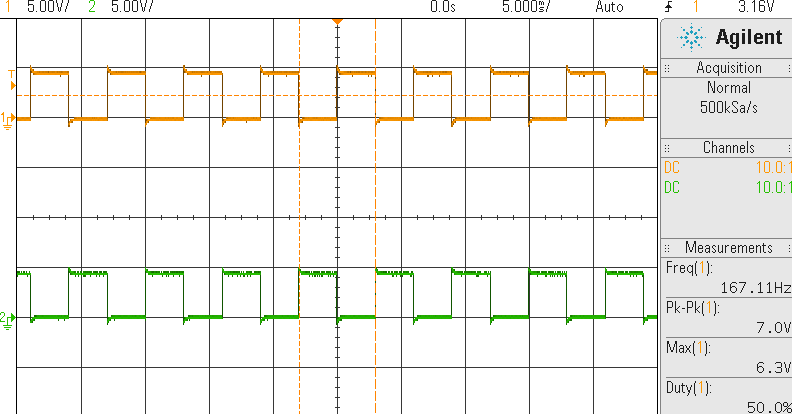
\includegraphics[width=1\textwidth]{max_trans_outputAB.png}
            \vspace{-8mm}
            \caption{\small{A and B output transmitted}}
        \end{figure}
      \end{minipage}\\
      &\\
      \hline
    \textbf{\underline{{Reception test}}} & \\
    \vspace{-5mm}
    \begin{minipage}[b]{0.45\textwidth}
    \begin{figure}[H]
        \centering
        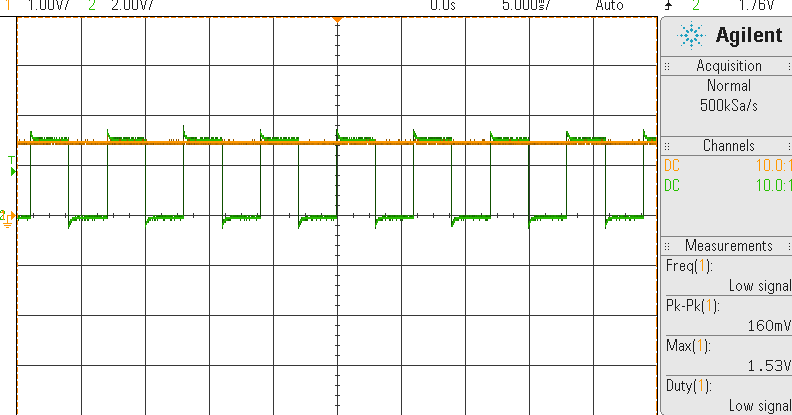
\includegraphics[width=1\textwidth]{max_recieve_signal.png}
        \vspace{-8mm}
        \caption{\small {Signal being received}}
    \end{figure}
    \end{minipage}
    &
    \begin{minipage}[b]{0.45\textwidth}
    \begin{figure}[H]
        \centering
        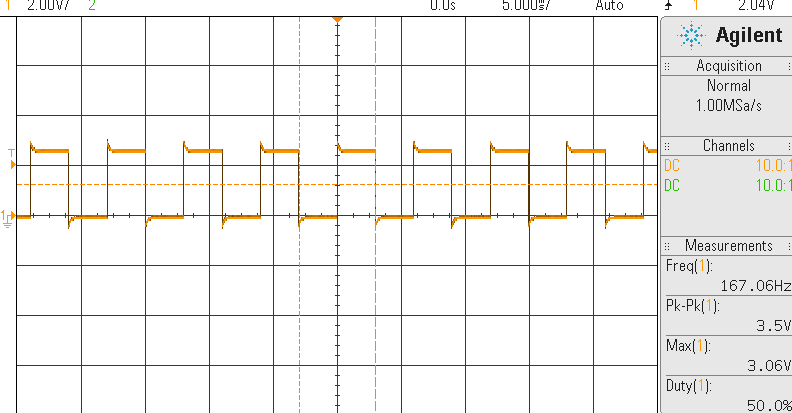
\includegraphics[width=1\textwidth]{max_receive_output.png}
        \vspace{-8mm}
        \caption{\small{RO received signal}}
    \end{figure}
    \end{minipage}\\
    &\\
    \hline
    \end{tabular}
    \caption{Caption}
\end{table}
\vspace{-5mm}




\newpage
\section{Buck Converter}
The data sheet for the LM5088 includes a typical setup for this particular buck converter. It goes through each step in the design procedure as well as all the equations needed to solve for all the necessary resistor and capacitor values as well as any other needed components that are required to run the buck converter.

Texas Instruments online power supply designer, WeBench was used to choose the buck converter chip and components required to produce the required output voltage.

The chosen buck converter design consisted of only surface mount components. The buck converter chip has a thermal pad at its base and with 16 pins it made it impossible to assemble the buck converter for testing.

Though it can be assumed that the designed buck converter works as Texas Instruments is reliable supplier of electronic equipment and components.




\newpage
\section{Voltage Regulator}
The MCP9700 chip was connected to 5V and Ground. The output voltage was then measured at the output pin. 

The regulator stability was then tested for various current draws using a resistor bank as a load. The results can be seen below in Table 4.6.

\begin{table}[H]
\centering
    \begin{tabular}{|c| c| c|}
    \hline
    \textbf{\underline{Load resistance (\ohm)}}  & \textbf{\underline{$I_{out}$ (mA)}} & \textbf{\underline{Vout (V)}}\\
       1k\ohm   & 3.3  & 3.28\\
       500\ohm  & 6.6  & 3.32\\
       250\ohm  & 13.2 & 3.35\\
       200\ohm  & 16.5 & 3.33\\
       125\ohm  & 26.4 & 3.37\\
       100\ohm  & 33   & 3.38\\
   \hline
    \end{tabular}
    \caption{Voltage load stability}
\end{table}
Various input voltages were applied in order to test the stability of $V_{OUT}$ with a constant load. The results can be seen below in Table 4.7.

\begin{table}[H]
\centering
    \begin{tabular}{|c| c|}
    \hline
      \textbf{\underline{$V_{IN}$}}  & \textbf{\underline{Vout (V)}}\\
       2 & 2.2  \\
       3 & 2.8 \\
       4 & 3.35\\
       5 & 3.33\\
       6 & 3.37\\
       7 & 3.32\\
       8 & 3.28\\
      \hline
    \end{tabular}
    \caption{Voltage stability}
\end{table}
It was found that the voltage regulator functioned well for voltages above 2.5V and maintained a stable output voltage regardless of the change in input voltage.